\documentclass{article}

\usepackage[utf8]{inputenc}
\usepackage[russian]{babel}
\usepackage{multicol}
\usepackage[8pt]{extsizes}
\usepackage[papersize={17cm, 23cm}, left=8mm, top=-1mm, right=8mm, bottom=20mm]{geometry}
\usepackage{mathtools}
\usepackage{amsmath}
\usepackage{graphicx}
\graphicspath{{pictures/}}
\usepackage[usenames]{color}
\usepackage[most]{tcolorbox}
\usepackage{colortbl}
\usepackage{fancyhdr}
\pagestyle{fancy}
\fancyhf{}
\DeclareGraphicsExtensions{.png}
\usepackage{afterpage}
\fancyfoot[R]{39}

\begin{document}
\begin{multicols}{2}

\parindent0pt
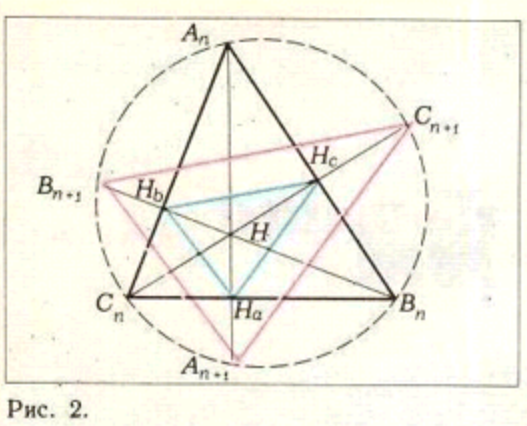
\includegraphics[scale=0.4]{ris2.png}

\parindent0pt
\scalebox{1.5}{%
Аналогично   получаем}

\parindent0pt
\scalebox{1.5}{%
$\angle$$\mathnormal{B_{n+1}=\mathrm{(-2)}^{n}\cdot}(\angle B_{1}-\frac{\pi}{3})+\frac{\pi}{3}$}\\
\scalebox{1.3}{%
и}\\
\scalebox{1.5}{%
$\angle$$\mathnormal{C_{n+1}=\mathrm{(-2)}^{n}\cdot}(\angle C_{1}-\frac{\pi}{3})+\frac{\pi}{3}$}\\

\parindent10pt
\scalebox{1.3}{%
В заключение мы предлагаем чи-}\\
\scalebox{1.3}{%
тателям несколько задач для само-}\\
\scalebox{1.3}{%
стоятельного решения.}\\

\parindent15pt
У п р а ж н е н и я

\parindent15pt
1. Около  остроугольного  треугольника\\
$\mathnormal{A_{1}B_{1}C_{1}}$ описан остроугольный треугольник\\
$\mathnormal{A_{2}B_{2}C_{2}}$, стороны которого являются каса-\\
тельными к окружности, описанной около\\
треугольника $\mathnormal{A_{1}B_{1}C_{1}}$ в его вершинах. Около\\
треугольника $\mathnormal{A_{2}B_{2}C_{2}}$ аналогичным образом\\
описан остроугольный треугольник $\mathnormal{A_{3}B_{3}C_{3}}$\\
и так далее, вплоть до треугольника\\
$\mathnormal{A_{n+1}B_{n+1}C_{n+1}}$ включительно. Найти углы\\
треугольника $\mathnormal{A_{n+1}B_{n+1}C_{n+1}}$.

\parindent15pt
2. Около треугольника $\mathnormal{A_{1}B_{1}C_{1}}$ описан\\
треугольник $\mathnormal{A_{2}B_{2}C_{2}}$ вершины которого сов-\\
падают с центрами вневписанных окружнос-\\
тей в треугольник $\mathnormal{A_{1}B_{1}C_{1}}$. Около треуголь-\\
ника $\mathnormal{A_{2}B_{2}C_{2}}$ аналогичным образом описан\\
треугольник $\mathnormal{A_{3}B_{3}C_{3}}$ и так далее. Найти уг-\\
лы треугольника $\mathnormal{A_{n+1}B_{n+1}C_{n+1}}$. Доказать,\\
что треугольник $\mathnormal{A_{n+1}B_{n+1}C_{n+1}}$ при неогра-\\
ниченном возрастании n стремится к пра-\\
вильному треугольнику.

\parindent15pt
3. Биссектрисы треугольника $\mathnormal{A_{1}B_{1}C_{1}}$\\
продолжены до пересечения с описанной\\
вокруг треугольника $\mathnormal{A_{1}B_{1}C_{1}}$ окружностью\\
соответственно в точках $\mathnormal{A_{2}, B_{2}, C_{2}}$. Бис-\\
сектрисы треугольника $\mathnormal{A_{2}B_{2}C_{2}}$ пересекают\\
описанную окружность соответственно в точ-\\
ках $\mathnormal{A_{3}, B_{3}, C_{3}}$ и так далее. Найти углы\\
треугольника $\mathnormal{A_{n+1}B_{n+1}C_{n+1}}$.

\parindent15pt
4. В треугольник $\mathnormal{A_{1}B_{1}C_{1}}$ вписан тре-\\
угольник $\mathnormal{A_{2}B_{2}C_{2}}$ образованный проекция-\\
ми центра вписанной окружности на его сто-\\
роны. В треугольник $\mathnormal{A_{2}B_{2}C_{2}}$ аналогичным\\
образом вписан треугольник $\mathnormal{A_{3}B_{3}C_{3}}$ и\\
так далее. Найти углы треугольника\\
$\mathnormal{A_{n+1}B_{n+1}C_{n+1}}$. \\ \\

%\begin{left}
%\end{left}

\parindent0pt
\scalebox{2}{%
Головоломки}\\

\scalebox{1.3}{% 
В следующих примерах раз-}\\
\scalebox{1.3}{% 
ные цифры зашифрованы раз-}\\
\scalebox{1.3}{% 
ными буквами (в разных}\\
\scalebox{1.3}{% 
примерах, возможно, раз-}\\
\scalebox{1.3}{% 
ными). Расшифруйте!}

\parindent15pt
\scalebox{1.3}{%
1. do$\times$ do $=$ sol.}

\parindent15pt
\scalebox{1.3}{%
2. la$\times$la $=$ sol.}

\parindent15pt
\scalebox{1.3}{%
3. си$\times$си $=$ соль. }

\parindent15pt
\scalebox{1.3}{%
4. до$\times$до$\times$до $=$ соль. }

\parindent15pt
\scalebox{1.3}{%
5. ля$\times$ля$\times$ля $=$ соль. } 

\parindent50pt
\scalebox{1.3}{%
\textit{В. С. Максимов} } \\ \\

\parindent0pt
\scalebox{2}{%
Равенства}\\ \\
\scalebox{2}{%
из спичек}\\

\parindent0pt
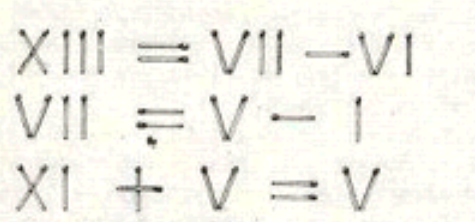
\includegraphics[scale=0.4]{sp.png}

\scalebox{1.3}{%
В этих равенствах, сло-}\\
\scalebox{1.3}{%
женных из спичек, допущены}\\
\scalebox{1.3}{%
ошибки. Переложите в каж-}\\
\scalebox{1.3}{%
дом из равенств только по}\\
\scalebox{1.3}{%
одной спичке так, чтобы все}\\
\scalebox{1.3}{%
равенства стали верными.}

\parindent50pt
\scalebox{1.3}{%
\textit{Н. К. Антонович} } \\ \\

\parindent0pt
\scalebox{2}{%
Задачи}\\ \\

\parindent15pt
\scalebox{1.3}{%
1. Решить     уравнение
}\\
\parindent0pt
\scalebox{1.3}{%
$x^{4}-3x^{3}+3=0$.
}

\parindent15pt
\scalebox{1.3}{%
2. Показать, что при лю-}

\parindent0pt
\scalebox{1.3}{%
бом действительном $р$ таком,}\\
\scalebox{1.3}{%
что $|p|\leq \sqrt[4]{4q}$, уравнение}\\
\scalebox{1.3}{%
$x^{4}+px^{3}+q=0$, $q > 0$}\\
\scalebox{1.3}{%
действительных решений не}\\
\scalebox{1.3}{%
имеет.}

\parindent15pt
\scalebox{1.3}{%
3. Показать, что при лю-}

\parindent0pt
\scalebox{1.3}{%
бом действительном $р$ таком,
}\\
\scalebox{1.3}{%
что $|p|\leq \sqrt[4]{12}$, уравнение}\\
\scalebox{1.3}{%
$x^{4}-px^{3}+3=0$}\\
\scalebox{1.3}{%
действительных решений не}\\
\scalebox{1.3}{%
имеет.}

\parindent15pt
\scalebox{1.3}{%
4. Найти действитель-}

\parindent0pt
\scalebox{1.3}{%
ные решения системы}\\
\scalebox{1.3}{%
$x^{3}y = -4$, $x - y = 1,5$.}

\parindent60pt
\scalebox{1.3}{%
\textit{Г. Ю. Зайцев}}

\end{multicols}
\end{document}